\documentclass[preview]{standalone}

% pgfplots
\usepackage{pgfplots}
\pgfplotsset{compat=newest}
\usepackage{xcolor}
\usepackage{blkarray}
\usepackage{tikz-network}
\usepackage{graphicx}
\usepackage{float}
\usepackage{caption}
\usepackage{subcaption}
\usetikzlibrary{
    arrows.meta,
    matrix,
    positioning,
    patterns,
}
\begin{document}
\begin{figure}[!htb]
    \centering
    \begin{subfigure}[b]{1.0\textwidth}
        \centering
        \begin{tikzpicture}
            \Vertices{data/graphs/ex1/vertices.csv}
            \Edges{data/graphs/ex1/edges.csv}
        \end{tikzpicture}
        \caption{}
    \end{subfigure}

    \begin{subfigure}[b]{0.3\textwidth}
        \centering
        \begin{blockarray}{c|ccccc}
            & A & B & C & D & E \\
            \BAhline
            \begin{block}{c|ccccc}
                A & 0 & 3 & 5 & 0 & 3 \\
                B & 3 & 0 & 3 & 0 & 0 \\
                C & 0 & 0 & 0 & 2 & 0 \\
                D & 0 & 0 & 2 & 0 & 3 \\
                E & 3 & 0 & 0 & 3 & 0 \\
            \end{block}
        \end{blockarray}
        \caption{}
    \end{subfigure}
    \hspace{3em}
    \begin{subfigure}[b]{0.3\textwidth}
        \centering
        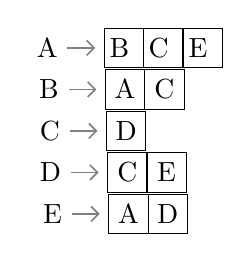
\begin{tikzpicture}[
                node distance = 21mm and 7mm,
                box/.style = {draw, minimum size=5mm, inner sep=0pt, outer sep=0pt, anchor=west},
                pin edge = {Straight Barb-, shorten <=1mm,semithick}
            ]
            \matrix (mat1) [matrix of nodes,
                nodes={box},
                align=left,
                column sep=-\pgflinewidth,
                inner sep=0pt,
                pin=180:A
            ]
            {
                B & C & E \\
            };
            \matrix (mat2) [matrix of nodes,
                below=1.5em of mat1-1-1.west,
                anchor=west,
                nodes={box},
                column sep=-\pgflinewidth,
                inner sep=0pt,
                pin=180:B
            ]
            {
                A & C \\
            };
            \matrix (mat3) [matrix of nodes,
                below=1.5em of mat2-1-1.west,
                anchor=west,
                nodes={box},
                column sep=-\pgflinewidth,
                inner sep=0pt,
                pin=180:C
            ]
            {
                D \\
            };
            \matrix (mat4) [matrix of nodes,
                below=1.5em of mat3-1-1.west,
                anchor=west,
                nodes={box},
                column sep=-\pgflinewidth,
                inner sep=0pt,
                pin=180:D
            ]
            {
                C & E \\
            };
            \matrix (mat5) [matrix of nodes,
                below=1.5em of mat4-1-1.west,
                anchor=west,
                nodes={box},
                column sep=-\pgflinewidth,
                inner sep=0pt,
                pin=180:E
            ]
            {
                A & D \\
            };
        \end{tikzpicture}
        \vspace{1em}
        \caption{}
    \end{subfigure}
\end{figure}
\end{document}